% Caso de estudio 1: Machine Learning — Cotización de fletes · Gravetal Bolivia
% Compilar: pdflatex informe_final.tex (dos pasadas).
\documentclass[11pt]{article}
\usepackage[utf8]{inputenc}
\usepackage[spanish]{babel}
\usepackage[a4paper,margin=2cm,top=2.3cm,bottom=2.3cm]{geometry}
\usepackage{tgheros}
\renewcommand{\familydefault}{\sfdefault}
\usepackage{xcolor}
\usepackage{booktabs}
\usepackage{enumitem}
\usepackage{titlesec}
\usepackage{fancyhdr}
\usepackage{tcolorbox}
\usepackage{multicol}
\usepackage{graphicx}
\usepackage{amssymb}
\usepackage{hyperref}
\definecolor{gravetal}{HTML}{153C5A}
\definecolor{acento}{HTML}{00A7C6}
\definecolor{alerta}{HTML}{D97008}
\definecolor{fondo}{HTML}{F2F7FC}
\setlist{itemsep=2pt,topsep=2pt,parsep=0pt}
\titleformat{\section}{\Large\bfseries\color{gravetal}}{}{0em}{}[\vspace{-1ex}\rule{\linewidth}{1.2pt}]
\titleformat{\subsection}{\bfseries\color{gravetal}}{}{0em}{}
\pagestyle{fancy}
\fancyhf{}
\fancyhead[L]{\small\textsc{Caso de estudio 1 · Machine Learning}}
\fancyfoot[R]{\small Pág. \thepage}
\fancyfoot[L]{\small\textsc{Gravetal · Informe final · Oct-2026}}
\renewcommand{\headrulewidth}{0.6pt}
\hypersetup{colorlinks=true,linkcolor=gravetal,urlcolor=acento}
\graphicspath{{./}}
\newtcolorbox{kpi}{colback=fondo,colframe=acento,boxrule=1pt,arc=3mm,
  fontupper=\bfseries\color{gravetal},halign=center,valign=center}
\newcommand{\blank}[1]{\par #1: \rule{9cm}{0.4pt}\par\vspace{0.6ex}}
\begin{document}
% ---------- CARÁTULA (una hoja) ----------
\thispagestyle{empty}
\begin{center}
\includegraphics[height=2.8cm]{"logo umsa"}\\[1ex]
{\small\textsc{Universidad Mayor de San Andrés}}\\[2ex]
{\color{acento}\rule{\linewidth}{2pt}}\\[2ex]
{\Huge\bfseries\color{gravetal} Caso de estudio 1:\\ Machine Learning}\\[1.5ex]
{\large Cotización inteligente de fletes de exportación · Gravetal Bolivia}\\[0.5ex]
{\small Metodología CRISP-DM · Modelo Ridge en producción · Snowflake + Python + App offline}
\end{center}
\vspace{2ex}
\blank{Materia}
\blank{Docente}
\blank{Dupla 2 — Integrante 1}
\blank{Dupla 2 — Integrante 2}
\vspace{1ex}
\begin{center}
\begin{minipage}{0.31\linewidth}\begin{kpi}R² 0.905\\{\small test}\end{kpi}\end{minipage}\hfill
\begin{minipage}{0.31\linewidth}\begin{kpi}MAE \$26.55\\{\small test}\end{kpi}\end{minipage}\hfill
\begin{minipage}{0.31\linewidth}\begin{kpi}MAPE 16\%\\{\small test}\end{kpi}\end{minipage}
\end{center}
\vfill
\begin{center}{\small v1 · Octubre 2026 · rama \texttt{mineria} ·
\texttt{Despligue/app\_flete.html} + \texttt{modelo\_flete\_web.json}}\end{center}
\newpage
% ---------- ÍNDICE ----------
\section*{Índice y control documental}
\begin{multicols}{2}
\begin{enumerate}[leftmargin=*]
\item Comprensión del negocio (CRISP-DM 1)
\item Datos y dataset (CRISP-DM 2 · Crit. 1)
\item Análisis de variables (Crit. 11)
\item Preparación: train / test (CRISP-DM 3 · Crits. 2--3)
\item Modelado (CRISP-DM 4 · Crit. 5)
\item Validación (Crit. 9)
\item Métricas y resultados (CRISP-DM 5 · Crits. 4 y 7)
\item Visualizaciones (Crit. 8)
\item Valor para el negocio (Crit. 6)
\item Datos en la nube (Crit. 10)
\item Despliegue (CRISP-DM 6)
\item Monitoreo y mantenimiento (CRISP-DM 6)
\item Cierre, futuro y anexos
\end{enumerate}
\end{multicols}
\subsection*{Control de versiones}
\begin{tabular}{lll}
\toprule Versión & Fecha & Cambio \\
\midrule v1 & Oct-2026 & Ridge $\alpha{=}0.1$, MAE \$26.55, $R^2$ 0.905, app verificada 5/5 \\
\bottomrule
\end{tabular}
\subsection*{Cómo leer este informe}
Cada capítulo mapea una fase CRISP-DM y los 11 criterios del programa Python.
Los gráficos se generaron con matplotlib desde los resultados medidos.
% ---------- RESUMEN ----------
\section{Resumen ejecutivo}
Gravetal exporta harina y aceite de soya; el flete define gran parte del margen.
Este proyecto convierte 20\,000 envíos históricos en un \textbf{cotizador supervisado}
con \textbf{MAE \$26.55 y $R^2$ 0.905}, 74.1\% mejor que el baseline de la media.
\begin{center}
\begin{minipage}{0.31\linewidth}\begin{kpi}74.1\%\\{\small mejora vs media}\end{kpi}\end{minipage}\hfill
\begin{minipage}{0.31\linewidth}\begin{kpi}17\,000\\{\small filas train}\end{kpi}\end{minipage}\hfill
\begin{minipage}{0.31\linewidth}\begin{kpi}5/5\\{\small réplica JS $\checkmark$}\end{kpi}\end{minipage}
\end{center}
\begin{itemize}[leftmargin=*]
\item \textbf{Entrega:} modelo Ridge verificado + app HTML offline (predicción, lotes CSV, dashboards, monitoreo).
\item \textbf{Garantía:} split cronológico 70/15/15, validación temporal de 3 folds, réplica JS vs sklearn 5/5 (diff $<0.01$).
\item \textbf{Valor:} cotización en segundos con banda $\pm1$ MAE (\$53.10 de ancho); re-entrenamiento si MAE mensual $>\$35$ o deriva $>15\%$.
\item \textbf{Honestidad:} sintéticos en cuarentena (contrato 1, ventas 2025, fechas 1990/2099) y frentes nulos documentados (calidad AUC$\approx$0.5, retrasos $R^2\approx$0).
\end{itemize}
% ---------- NEGOCIO ----------
\section{Comprensión del negocio (CRISP-DM 1)}
\textbf{Objetivo:} reducir el error de cotización para proteger el margen del crush
($\approx$80 USD/TN). \textbf{Traducción:} regresión del \texttt{costo\_flete\_usd}
con 8 features de ruta, equipo y mes. Métrica principal MAE (dólares); secundarias $R^2$ y MAPE.
\begin{center}
\begin{minipage}{0.31\linewidth}\begin{kpi}MAE $<\$35$\\{\small logrado \$26.55 $\checkmark$}\end{kpi}\end{minipage}\hfill
\begin{minipage}{0.31\linewidth}\begin{kpi}{$R^2>0.80$}\\{\small logrado 0.905 $\checkmark$}\end{kpi}\end{minipage}\hfill
\begin{minipage}{0.31\linewidth}\begin{kpi}{MAPE $<20\%$}\\{\small logrado 16\% $\checkmark$}\end{kpi}\end{minipage}
\end{center}
\textbf{Decisión que habilita:} cotizar un embarque en segundos con banda de confianza
en vez de estimar a mano (error $>\$100$). Regla: banda superior bajo el precio del
cliente $\to$ cerrar; si la cruza $\to$ renegociar ruta/mes/transporte o escalar.
% ---------- DATOS ----------
\section{Datos y dataset (CRISP-DM 2 · Criterio 1)}
\textbf{Origen:} Snowflake \texttt{WMNAMCT-LN60692 / ARQUI1.CAPA\_BRONCE},
\texttt{ENVIO} + \texttt{TRANSPORTE} unidas por \texttt{ID\_TRANSPORTE}, vía
\texttt{COMPUTE\_WH}. Una sola query con JOIN + filtro ($>0$); sin credenciales en código.
{\small
\begin{center}
\begin{tabular}{llll}
\toprule Variable & Tipo & Rol & Calidad \\
\midrule distancia\_km & numérica & feature & $>0$; media train 1483.4 \\
duracion\_h & numérica & feature & de fechas; media 9.38 \\
capacidad\_tn & numérica & feature & media 412.2; atípicos vigilados \\
mes & 1--12 & feature & estacionalidad de campaña \\
tipo / origen / destino / bandera & categóricas & features & 4 / 3 / 5 / 4 niveles; nulos $\to$ FALTA \\
costo\_flete\_usd & numérica & \textbf{target} & $>0$; sin leakage a features \\
\bottomrule
\end{tabular}
\end{center}}
EDA: 20\,000 filas útiles; colas a la derecha (rutas largas caras); correlación
distancia--costo dominante; duplicados y outliers por rango; artefactos sintéticos en cuarentena.
% ---------- VARIABLES ----------
\section{Análisis de variables (Criterio 11)}
\begin{center}
\begin{minipage}{0.55\linewidth}
{\small
\begin{tabular}{lll}
\toprule Variable & Media & Lectura \\
\midrule distancia\_km & 1483.36 & Driver \#1 (coef. +8.76) \\
duracion\_h & 9.38 & Débil ceteris paribus \\
capacidad\_tn & 412.22 & Efecto escala leve \\
mes & 6.50 & Estacionalidad suave \\
\bottomrule
\end{tabular}}
\end{minipage}\hfill
\begin{minipage}{0.42\linewidth}
\begin{kpi}Distancia $\gg$ destino/origen $\gg$ resto\\{\small importancia del modelo}\end{kpi}
\end{minipage}
\end{center}
Niveles: tipo \{BARCAZA, CAMION, CAMION CISTERNA, FERROVIARIO\};
origen \{Puerto Quijarro, San Julián, Warnes\};
destino \{Buenos Aires, Puerto Aguirre, Puerto Quijarro, Rosario, Santos\};
bandera \{Argentina, Bolivia, Brasil, Paraguay\}. Sin multicolinealidad problemática
(Ridge la regulariza de todos modos).
% ---------- PREPARACIÓN ----------
\section{Preparación: train / test (CRISP-DM 3 · Criterios 2--3)}
\begin{itemize}[leftmargin=*]
\item \textbf{Limpieza:} costo$>0$, distancia$>0$; coerción a float; ``FALTA'' en nulos categóricos; sin imputar el target.
\item \textbf{Split cronológico 70/15/15} ($\approx$17\,000 train): respeta campañas; el test es el bloque final, nunca visto.
\item \textbf{Sin leakage:} mediana y estandarizado ajustados \textbf{solo en train}; one-hot con \texttt{handle\_unknown="ignore"}; $\alpha$ elegida solo en validación.
\item \textbf{Pipeline reproducible:} \texttt{SimpleImputer(median) $\to$ StandardScaler} + \texttt{OneHotEncoder} $\to$ Ridge; \texttt{random\_state} fijo; \texttt{scikit-learn==1.8.0}.
\end{itemize}
\begin{center}\begin{kpi}train (70\%) $\to$ validación temporal $\to$ test final intocable (15\%)\end{kpi}\end{center}
% ---------- MODELADO ----------
\section{Modelado (CRISP-DM 4 · Criterio 5)}
\textbf{Campeón: Ridge $\alpha{=}0.1$} (grilla logarítmica de 20 valores
$10^{-1}\dots10^{5}$): señal mayormente lineal + regularización del one-hot,
simple, estable y exportable a JSON exacto (20 coeficientes + intercepto 156.48).
\begin{center}
{\small
\begin{tabular}{llrr}
\toprule Modelo & Rol & MAE & Mejora vs media \\
\midrule Ridge & productivo & 26.55 & 74.1\% \\
HGB & retador & 26.41 & 74.2\% \\
RF & retador & 26.65 & 74.0\% \\
Media & baseline & 102.38 & --- \\
\bottomrule
\end{tabular}}
\end{center}
Solo ML supervisado (sin ARIMA por política; baselines ingenuos solo etiquetados).
Los tres ML empatan; Ridge queda por simplicidad y estabilidad.
% ---------- VALIDACIÓN ----------
\section{Validación (Criterio 9)}
TimeSeriesSplit de 3 folds en train para elegir $\alpha$; test evaluado una sola vez.
Train$\approx$test ($R^2$ 0.905): sin sobreajuste; +74.1\% vs baseline: capacidad suficiente.
\begin{center}
\begin{minipage}{0.46\linewidth}
{\small
\begin{tabular}{rrrr}
\toprule Caso & sklearn & JS & Diff \\
\midrule 1 & 368.44 & 368.44 & 0.001 \\
2 & 205.79 & 205.79 & 0.001 \\
3 & 242.86 & 242.86 & 0.003 \\
4 & 69.13 & 69.13 & 0.005 \\
5 & 71.99 & 71.99 & 0.005 \\
\bottomrule
\end{tabular}}
\end{minipage}\hfill
\begin{minipage}{0.50\linewidth}
\begin{kpi}Réplica exacta en navegador\\{\small diff máx 0.005 · 5/5 $\checkmark$}\end{kpi}
\end{minipage}
\end{center}
% ---------- EVALUACIÓN ----------
\section{Métricas y resultados (CRISP-DM 5 · Criterios 4 y 7)}
\begin{center}
\begin{minipage}{0.52\linewidth}
{\small
\begin{tabular}{lrrr}
\toprule Modelo (test) & MAE $\downarrow$ & $R^2$ $\uparrow$ & MAPE $\downarrow$ \\
\midrule \textbf{Ridge} & \textbf{26.55} & \textbf{0.905} & \textbf{16\%} \\
HGB & 26.41 & 0.903 & $\approx$16\% \\
RF & 26.65 & 0.901 & $\approx$16\% \\
Media & 102.38 & 0.000 & --- \\
\bottomrule
\end{tabular}}
\end{minipage}\hfill
\begin{minipage}{0.44\linewidth}
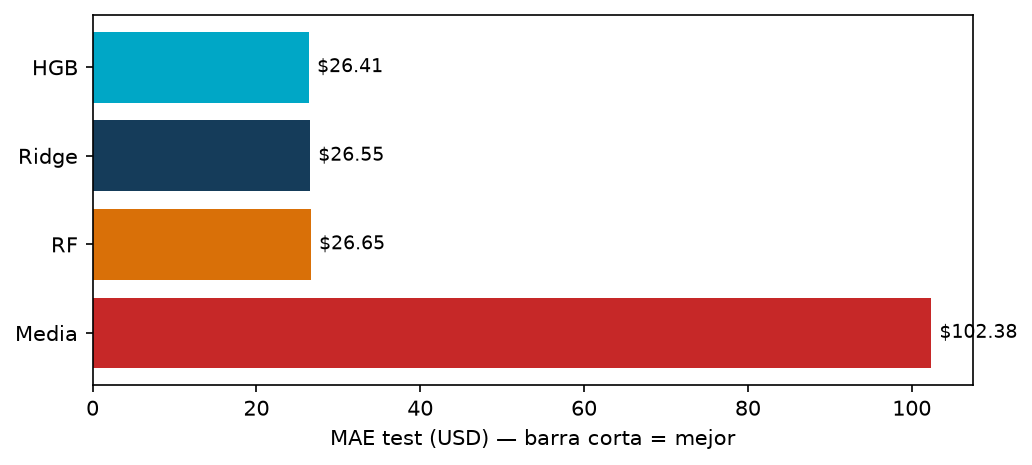
\includegraphics[width=\linewidth]{fig_duelo_mae}
\end{minipage}
\end{center}
Error típico $\pm\$26.5$ por envío (16\% relativo); 90.5\% de varianza explicada.
Cada cotización lleva banda $\pm1$ MAE (\$53.10 de ancho). Límites: rutas/países
nuevos $\to$ ``desconocido''; extremos fuera de rango $\to$ revisión humana.
\begin{center}
\begin{minipage}{0.62\linewidth}\centering{\small Ejemplo real: camión P. Quijarro $\to$ Rosario (1722 km)}
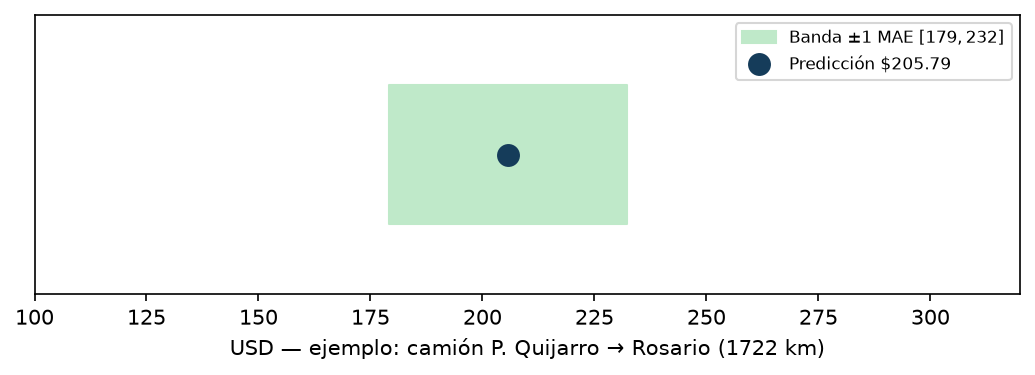
\includegraphics[width=\linewidth]{fig_banda}
\end{minipage}
\end{center}
% ---------- VIS ----------
\section{Visualizaciones (Criterio 8)}
\begin{center}
\begin{minipage}{0.48\linewidth}\centering{\small $R^2$ test por modelo (Media = 0, sin barra)}
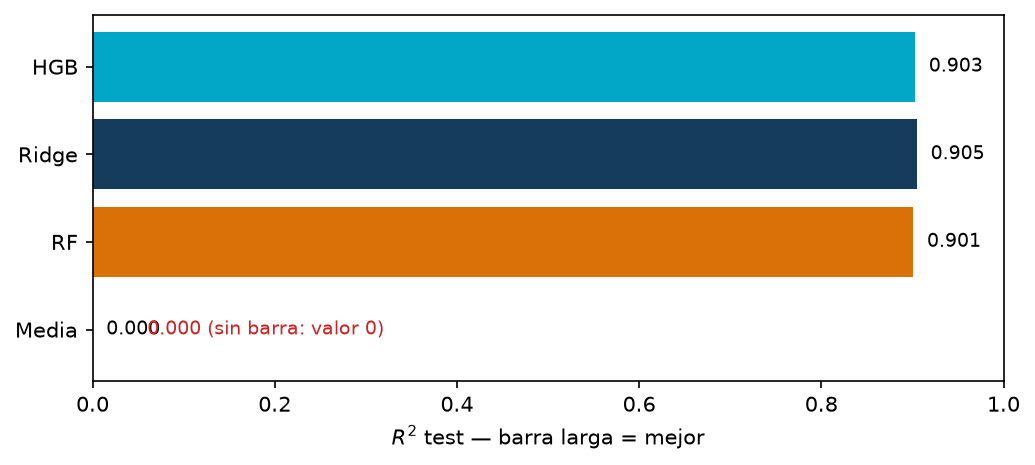
\includegraphics[width=\linewidth]{fig_r2}
\end{minipage}\hfill
\begin{minipage}{0.48\linewidth}\centering{\small Réplica sklearn vs JS (idénticas)}
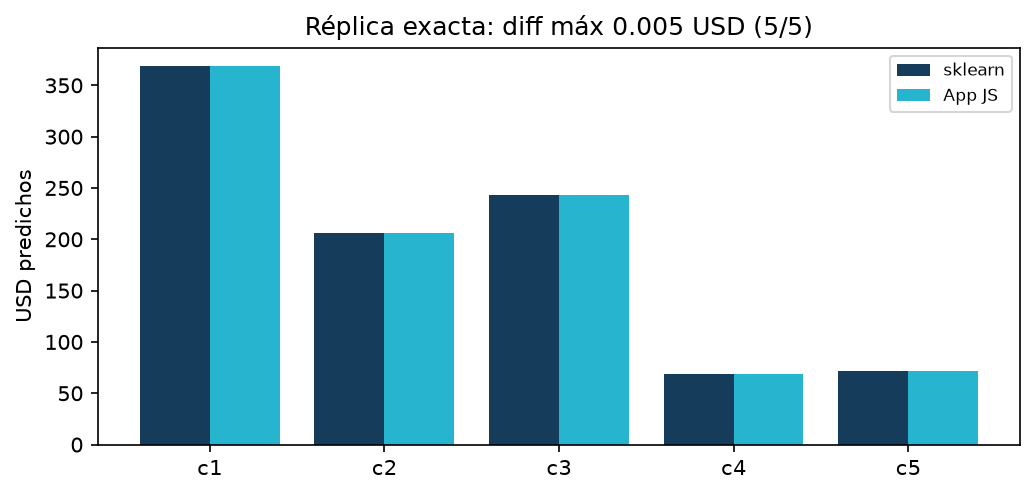
\includegraphics[width=\linewidth]{fig_casos}
\end{minipage}
\end{center}
\begin{center}
\begin{minipage}{0.72\linewidth}\centering{\small Frentes de apoyo: cobertura aceite e IoT térmico}
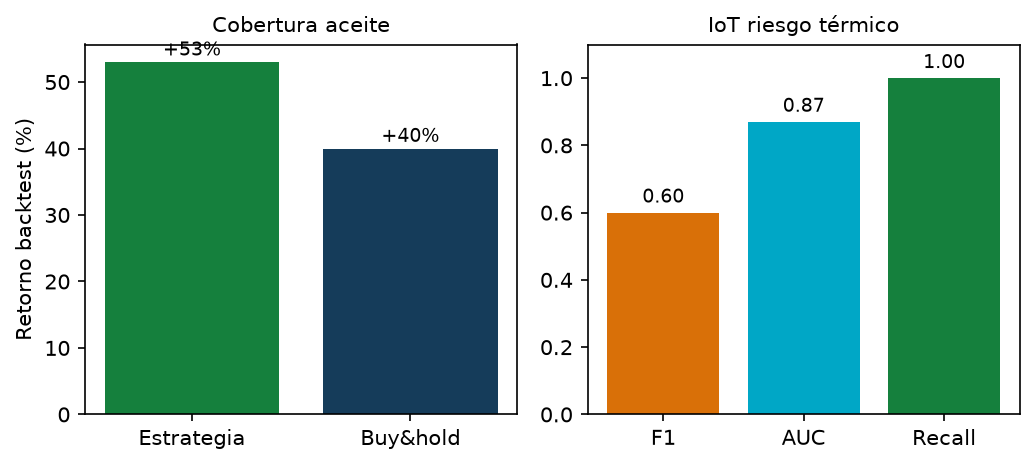
\includegraphics[width=\linewidth]{fig_negocio}
\end{minipage}
\end{center}
Gráficos matplotlib desde resultados medidos. La app suma gauge, donut, histograma
de lotes y banda $\pm$MAE por cotización.
% ---------- VALOR ----------
\section{Valor para el negocio (Criterio 6)}
\begin{itemize}[leftmargin=*]
\item \textbf{Cobertura aceite (backtest):} +53\% estrategia vs +40\% buy\&hold, vol $-$28\%, hit-rate 0.50 declarado: gestión de riesgo, no caja mágica.
\item \textbf{IoT térmico:} F1 0.60, AUC 0.87, recall $\approx$1.0 con sobre-alerta declarada.
\item \textbf{Ahorro indicativo:} de $\approx$\$102 a $\approx$\$27 de error medio $\approx$ \$75 por envío.
\end{itemize}
\begin{center}\begin{kpi}{$\approx$\$75\,000 de riesgo contenido}\\{\small 1\,000 envíos/año}\end{kpi}\end{center}
% ---------- NUBE ----------
\section{Datos en la nube (Criterio 10)}
\begin{center}
\begin{minipage}{0.55\linewidth}
\begin{itemize}[leftmargin=*]
\item Fuente \texttt{ARQUI1.CAPA\_BRONCE} (44/44 tablas, conteos idénticos).
\item Una query con JOIN + filtro vía \texttt{COMPUTE\_WH}.
\item Sin credenciales en código (sesión / entorno).
\item Scoring en navegador (sin servidor).
\end{itemize}
\end{minipage}\hfill
\begin{minipage}{0.42\linewidth}
\begin{kpi}{\texttt{modelo\_flete\_web.json}}\\{\small medianas · escalas · vocabularios · 20 coefs · $\alpha$ · métricas · 5 testigos}\end{kpi}
\end{minipage}
\end{center}
Re-entrenar = regenerar el JSON y republicar el HTML; el self-test 5/5 valida cada despliegue.
% ---------- DESPLIEGUE ----------
\section{Despliegue (CRISP-DM 6)}
\texttt{Despligue/app\_flete.html}: doble clic, sin internet, theme oscuro. Cuatro pestañas:
\begin{enumerate}[leftmargin=*]
\item \textbf{Predecir:} 8 campos (listas 4/3/5/4) $\to$ cotización con count-up, banda $\pm$MAE y top-3 factores del caso.
\item \textbf{Lotes CSV:} predice $N$ filas, MAE/$R^2$ si trae \texttt{costo\_flete\_usd}, histograma de 12 barras y descarga \texttt{predicciones\_flete.csv}.
\item \textbf{Dashboards:} KPIs con count-up, gauge $R^2$ 0.905, duelo MAE/$R^2$, cobertura, donut IoT, verificación 5 casos.
\item \textbf{Monitoreo:} deriva $>15\%$, registro v1, plan de mantenimiento y riesgos conocidos.
\end{enumerate}
Archivo de prueba: \texttt{Despligue/datos\_prueba\_fletes.csv} (12 envíos con costo; MAE simulado $\approx$\$9.5, estado ``sano'').
% ---------- MONITOREO ----------
\section{Monitoreo y mantenimiento (CRISP-DM 6)}
\begin{center}
{\small
\begin{tabular}{lll}
\toprule Señal & Regla & Acción \\
\midrule MAE mensual del lote & $>\$35$ dos meses & Re-entrenar y versionar (v2) \\
$R^2$ del lote & $<0.70$ & Declarar deriva, re-entrenar \\
Deriva de medias & $>15\%$ vs train & Revisar supuestos de ruta/precio \\
Esquema Bronce & columnas nuevas & Regenerar JSON + self-test 5/5 \\
\bottomrule
\end{tabular}}
\end{center}
\textbf{Riesgos vigilados:} ventas 2025 contaminadas (topes $<5000$/\,$<\$2000$),
contrato 1 e IDs basura, fechas 1990/2099, voltaje IoT constante 3.3.
\textbf{Registro:} v1 (29/9) Ridge $\alpha{=}0.1$, MAE \$26.55, $R^2$ 0.905, sklearn 1.8.0.
% ---------- CIERRE ----------
\section{Cierre, futuro y anexos}
\begin{multicols}{2}
\textbf{Conclusión:} cumple las tres metas, generaliza en test cronológico y opera
offline con réplica exacta; segunda opinión cuantificada, no orden automática.

\textbf{Limitaciones honestas:} calidad de grano (AUC$\approx$0.5, etiqueta aleatoria),
retrasos uniformes ($R^2\approx$0), IoT a 1 paso $\approx$ azar; sintéticos en cuarentena
no vuelven al train sin auditoría.

\textbf{Trabajo futuro:} intervalos conformales por ruta, features de
combustible/temporada, calibración mensual automática.

\textbf{Anexo — cuarentena:} productor 525 (4.381M TN) · contrato 1 ·
$\approx$800 ventas 2025 · fechas 1990/2099 · inventario $\gg$ capacidad · IoT 5 min.

\textbf{Glosario:} MAE = error absoluto medio (USD). $R^2$ = varianza explicada.
MAPE = error \%. Deriva = cambio de distribución vs train.
\end{multicols}
\end{document}
